\chapter{Data Acquisition}
\label{ch:sp-daq}

%%% todo

\fixme{\textbf{Authors:} 

  See \url{https://wiki.dunescience.org/wiki/Technical_Design_Report}
  for general guidance. 

  While this chapter is still in outline, \textbf{check that it hits all
  the required points} some of which are:

  We are to describe a \textbf{baseline} or \textbf{process to
  decide a baseline}.

  \textbf{BE SUCCINCT} $TDR \approx IDR + 10\%$, goal is 50 pages for
  this chapter. 

  You are encouraged to produce \textbf{tech notes} with any
  supporting verbosity which may be referenced.

  State requirements and demonstrate how they are met, use
  standardized requirements table.

  Emphasize safety and professionalism (projectisms: cost, schedule,
  risks, interfaces).}

\metainfo{Some sections of this chapter must be written generically
  and without any reference to module-specific terms. They are marked
  with an orange ``fixme'' box. 
  Yellow info boxes like this one provide guidance for the content. 
  This guidance is not comprehensive so authors may provide additional
  information but retaining \textbf{conciseness} and \textbf{not
    repeating} info in other section is required.}

\section{Introduction}
\label{sec:fd-daq:introduction}
% \fixme{module-generic}

% \metainfo{A brief introduction to this chapter describing what will be
%   described.  This is \textbf{not} an overview of the \dword{daq} itself.
%   Keep it brief. Do \textbf{not} write a conceptual overview here,
%   that is below, reference it. 
%   Do \textbf{not} use module-specific language but \textbf{do}
%   describe how commonalities are described in text shared by both
%   SP/DP volumes and specialized sections appear only in their
%   respective volume. 
%   \textbf{Do} describe the lexicographical convention used to demark
%   shared sections (this needs coordination with other chapters in the
%   same boat).}

The design of the \dword{dune} \dword{fd} \dword{daq} system is described in this chapter.  The \dword{daq} services all \dword{fd} \dwords{detmodule}.  Most  aspects of the design are identical across the different \dwords{detmodule} and are reproduced verbatim in sections of this \dword{daq} chapter from each \dword{detmodule} TDR volume.  A small part of the \dword{daq} design must be tailored to meet module-specific requirements and is documented in sections that are unique to each \dword{detmodule} TDR volume.  These sections are identified by their module-specific language.

The sections below begin with requirements for and interfaces between \dword{daq} and other \dword{dune} systems.  One section compares the \dword{protodune} experiment with \dword{dune} to highlight important information from the prototype and what must still be understood.  The subsequent section describes the design itself.  The chapter finishes with details on project management: production, installation, cost, schedule, safety, and other items.

\section{Requirements}
\label{sec:fd-daq:requirements}
\fixme{module-generic}

%\metainfo{One sentence introducing the contents of this section.}

The \dword{dune} \dword{fd} \dword{daq} system must meet the requirements 
summarized in Table~\ref{tab:fd-daq:requirements}. The system is
designed to meet these requirements and does so by following key
specifications provided in Section~\ref{sec:fd-daq:specifications}. 

\fixme{Add requirements table.}
%\input{generated/req-sp-daq.tex} 


%\fixme{The following are notes that need integration.}
%  \item Front-end Buffer sub-system shall provide sufficient continuous storage of the full detector data flow to allow for the delay needed by the Data Selection subsystem to form a trigger decision, for the resulting trigger command to be executed by the back-end Egress sub-system and for the selected data to be received by the back-end.
%  \item The Buffer sub-system shall further provide sufficient continuous storage of the full detector data flow to allow selecting a subset prior to an SNB trigger decision for a period of time indicated by current SBN models. 
 % This pre-trigger time is taken to be $\approx$10s.

 % \item The \dword{daq} shall minimize downtime for data acquisition and whenever possible continue nominal operations in parallel with any subset being taken offline or employed for any exceptional use.
%  \item Transitioning between \dwords{daqrun} shall require little to no downtime and shall require no downtime for \dwords{daqpart} unrelated to the transition.  
 
\subsection{Specifications}
\label{sec:fd-daq:specifications}
%\fixme{single-phase module}

Table~\ref{tab:fd-daq:specifications} lists
key specifications of the \dword{daq} design.  Some of the
specifications derive from the overall \dword{dune} \dword{fd} \dword{daq}
top level requirements.

%\item A \dword{daqrun} is identified with a \dword{daqrunnum}.
 % \item The components of the \dword{daq} shall be asynchronous and loosely coupled and in particular no global control of their state shall be centrally controlled.  Synchronization shall be performed dynamically and in a distributed fashion. 
 % \item The \dword{daq} shall be robust against intentional and unexpected removal and addition of individual components. 
  %  Single points of failure should not exist and may only be allowed based on a cost/risk analysis.
  %\item Detector coverage and \dword{daq} data selection criteria shall be recorded.  Coincident with intentional changes and upon discovery of unintentional changes the \dword{daq} shall transition to a new \dword{daqrun}.
 % \item Unexpected failures in the operation of \dword{daq} components should be automatically detected, reported, and handled so as to minimize system and human reaction time and to minimize reliance on human intervention.



%\metainfo{Include rows of top-level requirements table (``Schmitz''
% table) here. 
%  Augment that with any additional requirements of our determining. 
 % Eg: accept data from detector electronics, perform reduction to
 % satisfy output rate limit, allow for cross-module triggering,
 % collect beam activity with XX\%, SNB requirements, noise level,
  %total thermal and space envelop, etc....}
%
% \metainfo{Include message passing requirements and domains.}

\fixme{Add Specifications}

\begin{dunetable}
[Specifications for the \dword{dune} \dword{fd} \dword{daq} System.]
{cllc}
{tab:fd-daq:specifications}
{The \dword{dune} \dword{fd} \dword{daq} specifications, derived from
  the \dword{daq} top-level requirements.}  
Specification & Name & Description & Value \\ \toprowrule
% %THE FOLLOWING ARE selected from top level requirements, Nov. 5 version of xls sheet
%  8 & High-level Trigger & The \dword{daq} architecture shall provide a
%  parallel processing farm once events have been built to enhance data selection
%   capability and leverage the available bandwidth to permanent
%   storage. &  \\ \colhline
%  11 & Localization of trigger & The trigger system shall be capable of
%  recording the time and the aproximate APA location of each trigger for
% use in data reduction &  \\ \colhline
%  12 & Readout Data Buffering & Each readout shall store
%  data continuously in a ring so that when a trigger condition is
%  satisfied, the data from earlier (covering the trigger decision
%  latency and some additional lookback) is possible. & $>$\SI{4}{s}  \\
%  \colhline
% 13 & Trigger decision latency & The trigger decision time for single
%  interactions shall be made and delivered back to the continuous
% storage element within a time of 1s 99\% of the time and within 2s 100\%
% of the time and ALARA. & $<$\SI{1}{s} \\ \colhline
% 14 & Trigger window & The data around a trigger will be collected in a
% programmable time window that is configurable by trigger type.
% Excepting the SNB trigger (where data are writren to a different
% destination), this shall be programmable within a minimum time of 20us
% and a maximum of 30ms. & $<$\SI{20}{ms} \\ \colhline
% 15 & SNB trigger window & When a SNB trigger is activated, the data
% from the pre-trigger buffer and then the further incoming data shall
% be stored in a non-volatile solid-state-drive & \\ \colhline
% 16 & SNB deadtime & When the unallocated space in the SNB
% solid-state-drives runs out, the SNB trigger shall not
% overwrite existing data in the solid-state-drives. & \\ \colhline
% 17 & Livetime of triggers & A software programmable trigger priority
% scheme shall be provided, this shall be implemented in a way that the
% main physics triggers are never or rarely inhibited to enable the
% live-time of these triggers to be easilly determined. & \\
% \colhline
% 21 & Trigger primitives from APAs & A real-time algorith shall
% generate trigger primitives by search for "hits" on collection
% wires. Trigger Primitves will include information that is at least the
% channel number, the hit time, the pulse height or integral, and pulse
% width. Trigger Primitive generation will have a latency that is small
% enough that it can keep up with the detector data rate. & \\
% \colhline
% 22 & Trigger candidates from APAs & A real-time algorithm shall search
% for trigger candidates in each APA based on clustering of hit
% collection wires, total event charge, and pulse widths. "Low-energy"
% candidates will be identified for use in a supernova burst
% trigger. The latency from the processing time shall be small enough
% that candidate generation keeps up with data rate. & \\ \colhline
% 23 & Trigger Primitives from PDs & A real-time algorothm shall provide
% trigger primitives by searching for "hits" in photon detectors and
% provide. Trigger primitives will include at least channel number, hit
% time and pulse height information. The latency shall be small enough
% that it can keep up with detector data rate. & \\ \colhline
% 31 & Collection trigger primitives & The APA readout is currently only
% required to generate trigger primitives from the collection planes,
% and only on the wires facing the active detector. & \\
% 32 & Data compression & The APA readout may be losslessly compressed,
% but no general lossy compression should be applied.   The compression
% factor shall be at least 2. & 2 \\ \colhline
% 33 & Dead channels & Channels may be flagged by an operator as dead
% and the \dword{daq} shall disregard them in the trigger & \\ \colhline
% 34 & Noisy channels & Channels may be flagged by an operator as noisy
% and the \dword{daq} may disregard them in the trigger and apply a filtering
% before compression to improve compresibility of these channels & \\
%  101 & Supernova Deadtime Minimization & The \dword{daq} system shall allow
%  data collection to continue in some parts of the detector when a fault
%  or crash interrupts data collecting in one part. & \\ \colhline
%  102 & Remote operation & The data collection shall be controllable
%  easilly from remote locations and the authentication shall be
%  implemented to allow exclusive control. & \\ \colhline
%  103 & Expert mobile notification\/status & & \\ \colhline
%  105 & Combined Operation & The SP \dword{daq} shall be integrated fully with
%  and operate consistently to the DP \dword{daq} and the near detector \dword{daq} to
% allow shifts of all to be taken from one location by a small number of
% operators. & \\ \colhline
% 106 & Remote power and reset & Some form of slow control system & 
% \\ \colhline
% 111 & Partitioning & The \dword{daq} system shall permit concurrent runing of
% different subsets of the \dword{fd} elements in \dword{daqpart} to permit
% detector development or specialised runs in parallel with standard
% data taking. & \\ \colhline
% 112 & Data Flow Orchestrator & &  \\ \colhline
% 113 & Configuration & &  \\ 
\end{dunetable}

\subsection{Design Philosophy}

%\metainfo{Describe how the design addresses the requirements.}
The \dword{dune} \dword{fd} \dword{daq} addresses the requirements listed in
Section~\ref{sec:fd-daq:requirements}. The design itself facilitates a \dword{daq} system
that can be reconfigured and partitioned with great flexibility in implementing
\dword{daq} functionality in the system. 

Key philosophies are reflected in the design. The Readout sub-system is
designed so it can receive and buffer all raw data generated by
the full 10-kton module TPC and PDS systems with sufficient time to
facilitate O(1s)-latency triggers. The Data Selection sub-system
can process in real time raw data that meets data quality and noise
requirements with negligible dead time, providing
efficient triggering for the beam and non-beam physics program of
\dword{dune}. The adopted \dword{daq} partitioning scheme embodies a
highly configurable detector and maximizes the live time of the experiment while allowing for
reconfiguration, calibration, and debugging of subsets of the detector. 
%Add about The Control,
%Configuration and Monitoring design ...

The system is furthermore designed to be reconfigurable, flexible
enough to facilitate future design evolution and optimization,
including upgrades in FPGA and CPU data processing resources or
algorithm without changing the
overall data flow and processing architecture.

\subsection{Summary of Key Parameters}
\label{sec:sp-daq:parameters}
\fixme{single-phase module}

Table~\ref{tab:sp-daq:parameters} summarizes all important parameters
driving the \dword{daq} design.\fixme{This sentence simply repeats the table title. A little more discussion of the trends revealed in the table would help here, but obviously, that must wait for the values.}

%\metainfo{Include a table which lists all important parameters driving
%  the design.  Sampling rate and resolution, channel count}

\begin{dunetable}
[Key DAQ Parameters]
{cc}
{tab:sp-daq:parameters}
{Summary of important parameters driving the \dword{daq} design.}
Parameter & Value \\ \toprowrule
TPC Channel Count & \\ \colhline
PDS Channel Count & \\ \colhline
TPC Sampling Rate & \\ \colhline
& \\
\end{dunetable}

\section{Interfaces}
\label{sec:sp-daq:interfaces}
The \dword{dune} \dword{fd} \dword{daq} system interfaces with the TPC Cold Electronics, PDS
Readout, Computing, CISC, and Calibration systems of the \dword{dune}
\dword{fd}, as well as with Facilities and Underground Installation. The
interfaces are specified as interface agreements
and summarized in Table~\ref{tab:sp-daq:interfaces}. The system
interfaces are described in the following subsections. Interfaces with
Facilities and Underground Installation are described in Section~\ref{sec:sp-daq:production}.

%\metainfo{Include interface summary and table here.}

\begin{dunetable}
[DAQ System Interface Links]
{p{0.4\textwidth}p{0.2\textwidth}}
{tab:sp-daq:interfaces}
{Data Acquisition System Interface Links }
Interfacing System & Linked Reference \\ \toprowrule
TPC CE & \citedocdb{6742}\\ \colhline
PDS & \citedocdb{6727} \\ \colhline
Computing & \citedocdb{7123} \\ \colhline
CISC & \citedocdb{6790} \\ \colhline
Calibration & \citedocdb{7069} \\ \colhline
Timing & \citedocdb{11224} \\ \colhline
Facilities & \citedocdb{} \\ \colhline
Underground Installation & \citedocdb{} \\ 
\end{dunetable}

\subsection{TPC Cold Electronics}
The \dword{daq} and TPC Cold Electronics interface is described in \citedocdb{6742}.
\metainfo{Data reception physical and logical, configuration information delivery.}
\subsection{PDS Readout}
The \dword{daq} and PDS Readout interface is described in \citedocdb{6727}.
\metainfo{Data reception physical and logical, configuration information delivery.}
\subsection{Computing}
The \dword{daq} and Computing interface is described in \citedocdb{7123}.
\metainfo{Buffer disk.  Agreement on sysadmin support and computer procurement, ssh gateways, non data networks.  Address reference how the data model described above is acceptable.}
\subsection{CISC}
\label{sec:sp-daq:interfaces-cisc}
The \dword{daq} and CISC interface is described in \citedocdb{6790}.
\subsection{Calibration}
The \dword{daq} and Calibration interface is described in \citedocdb{7069}.
\subsection{Timing System}
Because the Timing System of the \dword{dune} \dword{fd} connects with
almost all detector systems and has a uniform interface to each of
them, rather than providing a set of 
bilateral interface documents, a single interface document
\citedocdb{11224} describes all timing interfaces. 

\section{\dword{protodune} and \dword{dune} Comparison}

\metainfo{Here we write what similarities and differences there are between \dword{protodune} and \dword{dune} \dword{daq} designs.}

\fixme{Notes:}
Differences between \dword{protodune} and \dword{dune} from Kurt's DFO and EB doc:
\begin{itemize}
\item Motivation: must accommodate changes in the overall system and provide more flexibility and granularity.
\item \dword{dune}: input to DFO is the trigger command, providing all space/time addressing required to identify the data to collect.  Information about the trigger decision itself is also included, but the DFO merely passes this through to output.  The addressing contains all information needed for the DFO to act.
\item \dword{dune}: The EB updates DFO about the resources (buffers) it has available.
\end{itemize}

\subsection{Detector Readout Hardware}

\metainfo{Compare and contrast design elements related to the detector readout hardware.}

\subsubsection{RCE}

\subsubsection{FELIX}

\subsection{Backend Event Building}

\subsection{Other}

\section{DAQ Design}
\label{sec:fd-daq:design}
% \fixme{module-generic}

% \metainfo{One sentence to introduce the section. 
%   Listing the subsections and describing which are generic and which
%   are X-phase specific.}

This section describes the \dword{daq} design. 
It begins with a conceptual overview followed by sections giving the design of the \dword{daq} subsystems. 
The \dword{ipc} and \dword{ccm} subsystems are described first.
Then the \dword{fe} data receiver and data handling and processing subsystems are covered.
Then, the subsystems for data selection and the \dword{daq} back-end are described. Finally, the timing subsystem is presented. The section finishes with plans for design validation and development.


The following descriptions of the design are brief. 
More details are provided as technical notes as listed in Table~\ref{tab:sp-daq:tech-notes}.

\begin{dunetable}{|p{0.7\textwidth}|p{0.2\textwidth}|}{tab:sp-daq:tech-notes}{Summary of relevant and detailed \dword{daq} technical notes.}
  Title & References \\
  \dword{dune} \dword{fd} Data Volumes & \citedocdb{9240}\\
  The \dword{daq} for the \dword{dune} prototype at CERN & \citedocdb{8708}\\
  A System for Communication Between \dword{daq} Elements & \citedocdb{10482}\\
  Data Selection for \dword{dune} Beam and Atmospheric Events & \citedocdb{11215}\\
  Data orchestrator and event building for \dword{dune} \dword{fd} \dword{daq} & t.b.d. \\
  \dword{dune} Run Control, Configuration \& Monitoring (CCM) & t.b.d. \\
  \dword{dune} \dword{daq} Readout & t.b.d. \\
\end{dunetable}



\subsection{Overview}
\label{sec:fd-daq:design-overview}
%\fixme{module-generic}

\begin{dunefigure}{fig:daq-conceptual-overview}{\dword{daq} Conceptual
    Subsystem Overview.  See text for description.}
  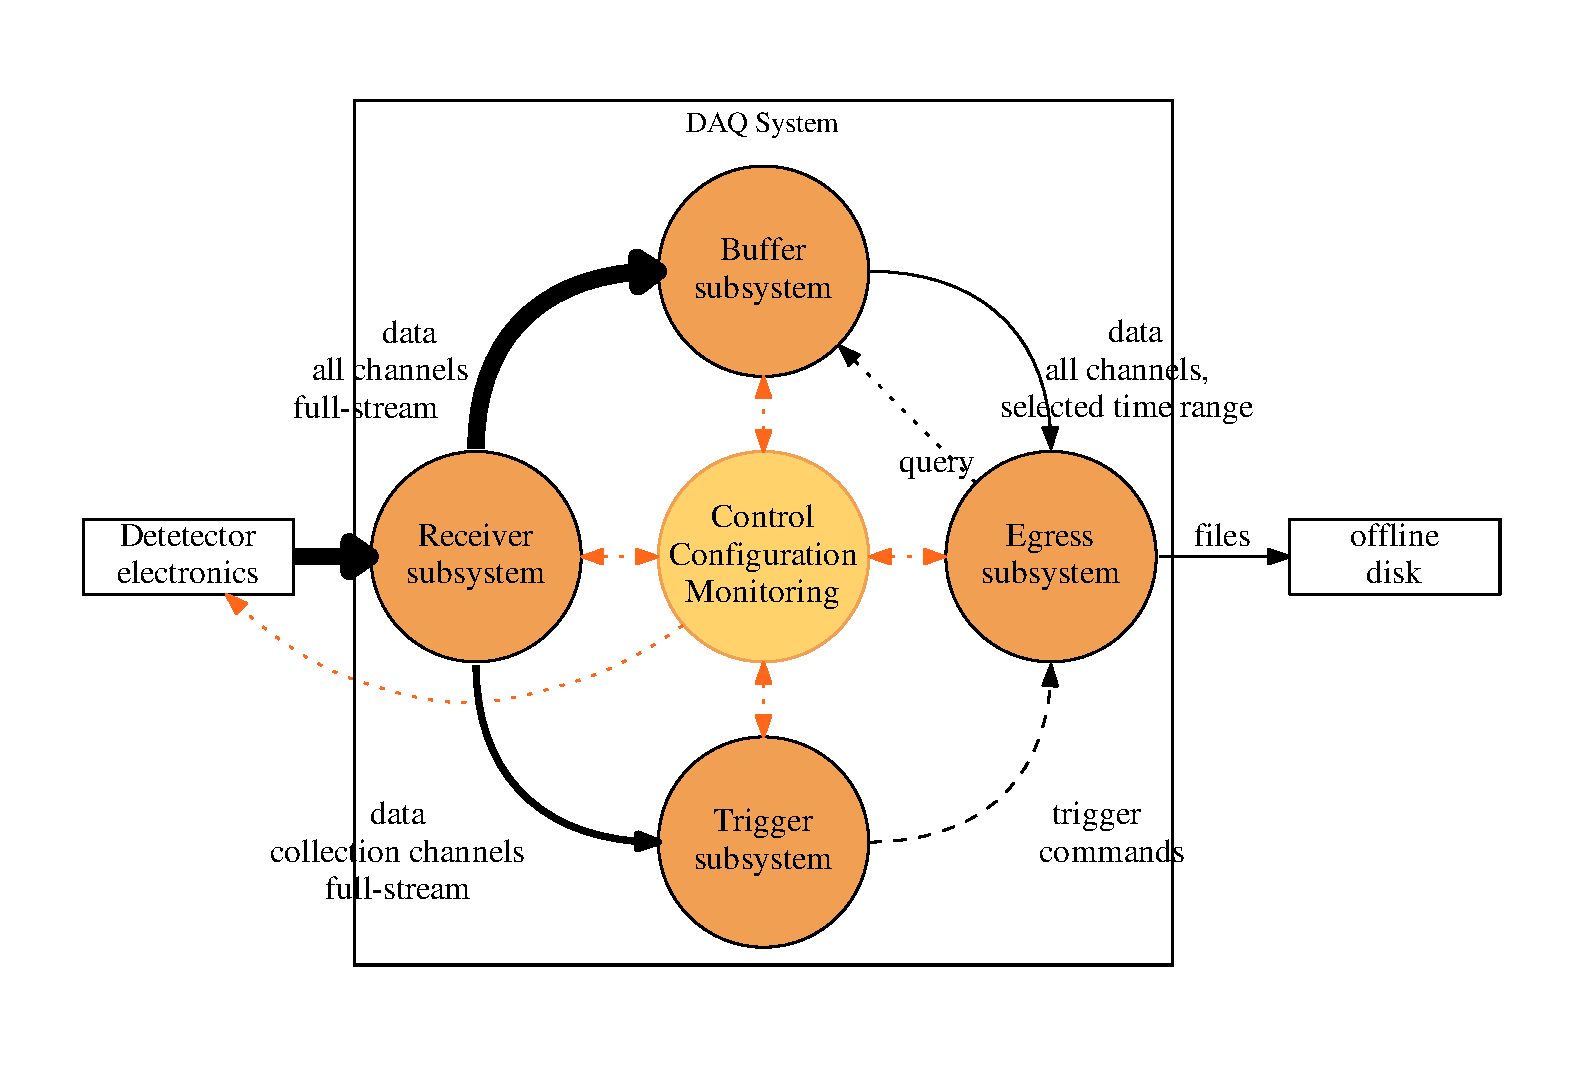
\includegraphics[width=0.8\textwidth]{daq-toplevel-conceptual.pdf}
\end{dunefigure}

% \metainfo{This is the \textbf{only} place to describe the conceptual
%   overview. 
%   Do \textbf{not} repeat this info in sections below. 
%   \textbf{Do} use \textbf{module-neutral} terms.
%   \textbf{Do} describe major interface between each subsystem (the edges between the circles in Fig~\ref{fig:daq-conceptual-overview}).
%   \textbf{Do} mention that concrete systems span portions of the
%   conceptual subsystems and how the following subsections are defined
%   along these concrete deliverable lines.}

Figure~\ref{fig:daq-conceptual-overview} provides an illustration of the conceptual parts that make up \dword{dune} \dword{fd} \dword{daq}. 
It applies to all \dword{fd} modules. 
The box in the illustration indicates the overall scope of the \dword{daq}.
Each of the concrete hardware and software subsystems described later in this section describe a portion of one or more of the conceptual subsystems represented by the circles in the figure.
Following the approximate data flow through the \dword{daq}, the concept starts with receiving input via optical fibers from the detector electronics (see Section~\ref{sec:fd-daq:design-felix}). 
The flow then bifurcates. 
The entirety of the input flow is buffered for sufficient time to satisfy triggering and readout requirements (see Section~\ref{sec:sp-daq:design-fe-processing}). 
The second flow need contain only data used to form a \dword{trigdecision} (see Section~\ref{sec:sp-daq:design-selection-algs}).
The egress subsystem uses the information in that decision to query the appropriate buffers and thus retrieve selected data (see Section~\ref{sec:fd-daq:design-backend}).
The results are aggregated and saved to files on nonvolatile storage media; custody is then transferred to offline responsibility.
This is all orchestrated by the \dword{ccm} subsystem (Section~\ref{sec:fd-daq:design-run-control}) shown in the center of the figure. The various information flows, represented by the arrows of the figure, ride on the \dword{ipc} subsystems (Section~\ref{sec:fd-daq:design-messages}). 

\metainfo{Include components summary and table here.  Need guidance on what is wanted.}

\fixme{Where will we describe partitions?}
As described more in Section~\ref{sec:fd-daq:partitions}, this conceptual picture is implemented through a number of \dwords{daqpart} or instances. 
The primary set of partitions will be underground in the \dword{cuc} for servicing the \dword{fd} modules. 
As described in Section~\ref{sec:sp-daq:production}, the \dword{daq} will connect to and begin servicing portions of \dword{fd} modules after they are installed and commissioned. 
A \dword{daq} presence will be kept in the \dword{itf} to support the work there during detector construction.
% \metainfo{Include physical location description}




\metainfo{For the remaining design sections: do not include directly validation info but rather place this information in Section~\ref{sec:sp-daq:design-validation} and make references.}
  



\subsection{Inter-process Communication}
\label{sec:fd-daq:design-messages}
\fixme{module-generic}

The \dword{daq} must transfer data between external sources and elements inside the \dword{daq}. 
These data are characterized using a variety of schema, latency, and throughput. 
The system that provides for such transfers is generally termed \dfirst{ipc}.
An IPC system consists of the following elements:
a set of message types, their data formats and schema,
a high-level, application protocol governing the exchange of its messages,
a set of supported message transport mechanisms, and
behavioral expectations for the participants in the message exchange. 


For the most part, the FD DAQ will require that supported transport mechanisms are reliable. 
Reliable here means that when one endpoint sends a message that it shall be received by the other endpoint even in the case of temporary loss of network connectivity or possibly temporary termination of the receiving endpoint.
The acceptable duration the broken connectivity is chosen based on the particular protocol in use.
Related to reliability, an IPC system may also provide behavior such as the \dword{daqdispre} function described in Section~\ref{sec:fd-daq:design-run-control}.

IPC, by design, is a system which interconnects diverse components and thus can encompass substantial complexity. 
In order to manage complexity and for practical reasons, the overall IPC system is segmented into a number of IPC \textit{domains}. 
In fact, certain \dword{daq} subsystems may require their own unique IPC implementation.
A single inter-domain IPC system will be developed for the FD DAQ. 
This system will provide a global \textit{lingua franca} communication between the domains. 
Some domains will also use this IPC for internal communications. 
A proxy service component will be developed to translate between the \textit{lingua franca} IPC and any domain which utilizes a unique IPC system.

The \textit{lingua franca} IPC, will be chosen after identifying options and evaluating them in terms of they features, performance, documentation and development simplicity. 
The selected IPC should also have an expectation of long term, and broad open source community support. 
The current candidate for a basis of the \textit{lingua franca} IPC is ZeroMQ. 
ZeroMQ provides a well established, high performance library. 
It has been positively evaluated by CERN~\cite{cern-zeromq}. 
It provides the basic building blocks for an IPC system in the form of high-level socket objects implementing a variety of socket patterns including publish/subscribe, exclusive pair, request/reply and others. 
Messages may be transported across thread-safe queues, Unix domain and network sockets which greatly assists in developing elastic applications that can scale from multi-threaded, multi-process and multi-computer contexts merely by changing configuration. 
The ZeroMQ ecosystem includes higher-level libraries providing for such important features as distributed discovery and presence (Zyre) as well as distributed configuration databases (Zgossip). 
Finally, it provides securely authenticated and authorized connections through elliptic curve public key encryption which will be useful for protecting some key communication against inadvertent connections.

One example of a subsystem that will likely utilize the \textit{lingua franca} IPC directly is the hierarchical trigger processing system provided by data selection (Section~\ref{sec:sp-daq:design-selection-algs}).
An example of a domain-specific IPC is that used by artDAQ that will be the heart of the egress subsystem as described in Section~\ref{sec:fd-daq:design-backend}.
The \dword{daq} will also interconnect with external domains. 
For example, a two-way exchange of information will exist between \dword{daq} and \dword{cisc}, as described in Section~\ref{sec:sp-daq:interfaces-cisc}.  

The \dfirst{ccm} subsystem (Section~\ref{sec:daq:design:ccm:control}) must communicate with all DAQ domains and in some cases directly to domain components and so is also expected to utilize the \textit{lingua franca} IPC. 
As described in that section, some of its functionality, particularly that of discovery and presence and zero-downtime reconfiguration, places requirements on the IPC.



\subsection{Control, Configuration, and Monitoring}
\label{sec:fd-daq:design-run-control}
% \fixme{module-generic}

% \metainfo{Describe run control and \dword{daq} operation monitoring. 
%   How it makes use of the Message Passing System. 
%   What is an ``epoch''.
%   How Epoch Change Requests lead to zero downtime reconfiguration. 
%   Public key based ``iron'' authentication between run control processes and the controlled processes. 
%   Describe how RC will configure partitioning, initiate reconfiguration, handle ``run'' changes, node discovery, configuration, logging, startup, shutdown and failures are handled. Describe how RC will support detector electronics configuration.}

\begin{dunefigure}{fig:daq-ccm-subsys}{Main interaction among the three CCM sub-systems.}
  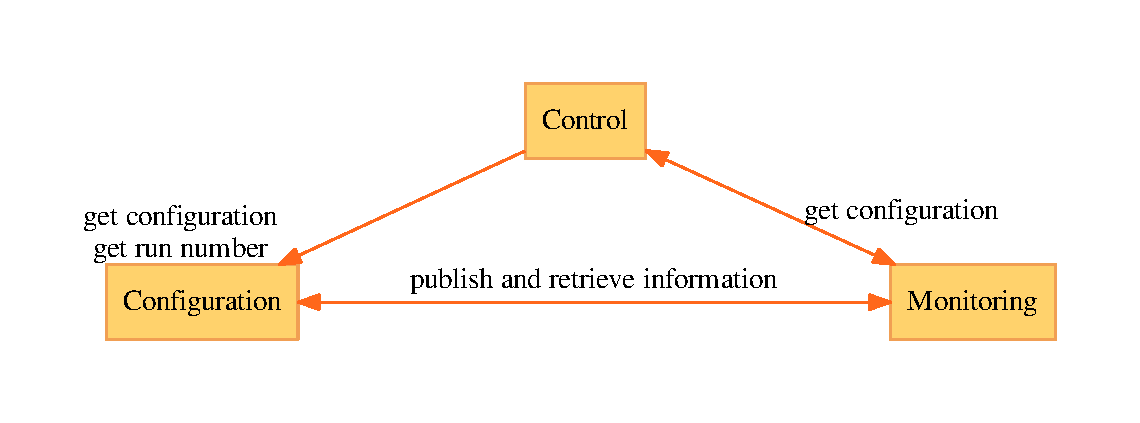
\includegraphics[width=0.8\textwidth]{daq-ccm-subsys.pdf}
\end{dunefigure}

The \dfirst{ccm} subsystem, illustrated in Figure~\ref{fig:daq-ccm-subsys}, encompasses, as it's name says, the software needed to control, configure, and monitor the rest of the \dword{daq} (as well as itself).
It provides a center for the highly distributed \dword{daq} components allowing them to be treated and managed as a coherent system. 
The CCM scope is high level in the sense that it does not directly handle the selection or transport of primary detector data but rather it handles (via IPC, see Section~\ref{sec:fd-daq:design-messages}) the sub-system components which provide these functions.
Figure~\ref{fig:daq-conceptual-overview} shows the central role of the \dword{ccm} within the complete \dword{daq} system.
The sub-systems of CCM are described in detail in the following sub-sections.


\subsubsection{Control}
\label{sec:daq:design:ccm:control}


The Control sub-system actively manages \dword{daq} software process lifetimes, asserts access control policies, executes commands, initiates configuration changes, detects and handles exceptions, and provides an interface for human operators.


% \fixme{I (bv) redrew this from Giovanna's to get vector PDF and match \dword{dune} color palette.  I made two content changes: 1: move UI out of partition as it can't both initiate a partition and be inside it and likely will allow for creation/viewing of more than just one partition.  2: I had to guess on how garbage collection might go and so addded a line from RM to PM. }

\begin{dunefigure}{fig:daq-ccm-control}{Roles and services which compose the \dword{daq} Control sub-system.}
  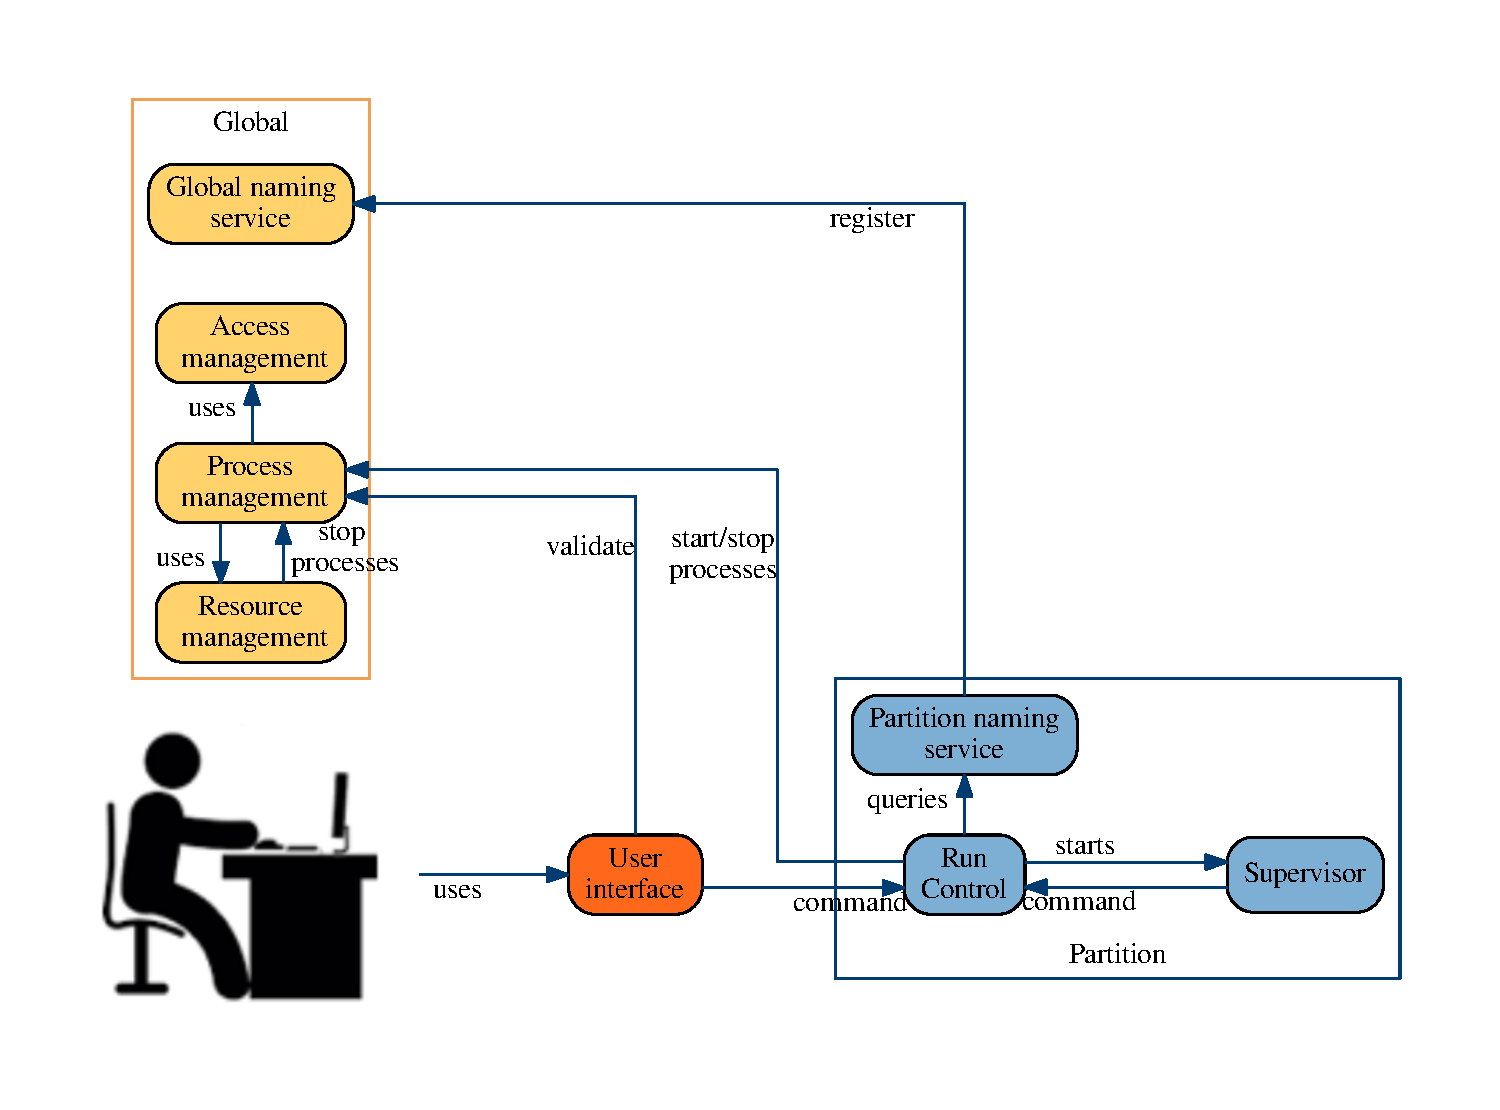
\includegraphics[width=0.8\textwidth]{daq-ccm-control.pdf}
\end{dunefigure}

The Control sub-sytem comprises a number of functional blocks of either global or partition scope as illustrated in Figure~\ref{fig:daq-ccm-control}. 
In the figure, ``partition'' refers to a logical segmentation of the DAQ where each segment operates to some extent independently from others. 
The segmentation applies to the portion of detector electronics providing input to the partition's data selection and readout. 
The largest partition would be that of one detector module.
The functional blocks in the figure represent one or more semi-autonomous agents, each with defined roles, capabilities, and access. 
Although drawn as single blocks, each are implemented as multiple peer agents to assure redundancy and fail-over. 
The blocks at partition scope are first described.

\begin{description}
\item[Partition naming service] provides \dword{daqdispre} for the components of a \dword{daqpart}. 
  That is, it allows a component to be made aware  of the creation and continued operation of other components (discovery) or that other components have recently become unresponsive (presence). 
  This service may be provided via distributed IPC mechanism or by an explicit, centralized (but redundant) service.

\item[Run control] provides a central director and its creation is the first step in initiating a \dword{daqpart}. 
  The \dword{rc} accepts, interprets, and validates input commands which may come either from a human via a user interface, or from other blocks. 
  The commands describe a desired state of the aggregate of all components that comprise the \dword{daqpart}. 
  \dword{rc} may query other blocks to validate commands and then execute the commands by allocating processes through process management. 
  Once successfully allocated, their lifetime is managed by \dword{rc}. 
  Throughout their lifetime, \dword{rc} may reconfigure existing processes, destroy them, or allocate additional processes. 
  \dword{rc} may query the partition naming service in order to resolve resource identifiers in commands into their corresponding network endpoint addresses.  

\item[Supervisor] provides a locus of expert system automation. 
  This block is initiated along with its \dword{rc} peer and augments human commands with automated ones. 
  For example, as certain ``common exceptions'' are encountered, understood and a means to correct them developed the supervisor can be extended to automatically issue the corrective actions that must otherwise be manually performed by a human operator.

\end{description}

Global scope controls \dword{daq} components for all \dwords{daqpart} across all \dword{fd} modules\footnote{\dword{daq} instances at locations other than the \dword{fd} cavern are expected to operate in a wholly distinct manner.}.  It consists of the following blocks:


\begin{description}
\item[Global naming service] aggregates the \dword{daqdispre} information across partitions.  Like the partition naming service, this may be implemented as a centralized (but redundant) explicit service or may be provided by extending the IPC \dword{daqdispre} mechanism to the entire FD DAQ network.

\item[Process management] allocates and may reclaim sets of processes on behalf of a requesting component (specifically \dword{rc} and resource management). 
  An allocation request includes a complete description of the processes and their desired initial configuration. 
  A successful allocation occurs only after this role successfully initiates all requested processes and confirms their presence. 
  Process management shall only allocate processes if their requester has appropriate access privileges as determined by access management and if resource management determines sufficient resources exist. 
  Process management may support pre-allocation if sufficient access and resources are confirmed and reserved; if so, a token (aka ``cookie'') is returned to the requester. 
  This cookie may be subsequently be presented to complete the allocation and claim the processes. 
  After a configured timeout, the cookie may be invalidated.\footnote{This will be required if the race condition between multiple UIs and RCs is a problem.}  
  
\item[Resource management] determines whether any process allocation can proceed and enacts a process garbage collection mechanism. 
  An allocation is successful if sufficient process resources are available and if it is consistent with a set of configured constraints maintained by this component. 
  Resource management monitors all allocated processes as well as the process initiating a request in order to perform ``garbage collection''. 
  This is performed in the event that the allocated processes outlive the requesting processes.
  Resource management shall notify process management of any remaining processes from an allocation when it detects that the requester is no longer present.
  Resource management shall also support pre-allocation validation queries. 
  A validation response merely indicates current state and it represents no guarantee that the allocation will subsequently succeed.

  
\item[Access management] is responsible for providing authentication and authorization for all \dword{daq} functions that require access control. 
  This block may be implemented as an explicit centralized (but redundant) service or through a distributed IPC mechanism or as some mixture of the two designs. 

\end{description}

The last block in Figure~\ref{fig:daq-ccm-control} represents applications that provide user interfaces (UI) to the control sub-system.
At least one UI will be developed to allow a trained operator to construct and issue commands required to initiate, configure, potentially reconfigure, and finally terminate \dwords{daqpart}. 
The UI may validate user commands before issuing them to an \dword{rc} by directly querying the process manager block. 
If sufficient resources are unavailable or if the user lacks appropriate access privileges, the UI will present a descriptive error message or otherwise disable corresponding functionality.  
If the user permission if valid the UI sends the use-initiated command to the \dword{rc} for execution.
Note that subsequent commands from the \dword{rc} to other blocks are also subject to access management.
Additional UI elements will be developed as described in sections~\ref{sec:daq:design:ccm:configuration} and~\ref{sec:daq:design:ccm:monitoring}.


\subsubsection{Configuration}
\label{sec:daq:design:ccm:configuration}

The \dword{daq} configuration sub-system provides persistent data storage for all historic, current, and future configuration information applicable to the \dword{daq}.
Further, it will provides a singular (but redundant) service for the allocation of unique and monotonically increasing \dwords{daqrunnum}.
The configuration data stores are operated in an insert-only mode. 
They do not support updating nor deleting previous records.
Configuration sub-system  shall support storing the following types of information:

\begin{description}

\item[Partition structure] contains descriptions of the multiplicity and connectivity of \dword{daq} components for any partition. 
  Structure and connectivity is expressed in an abstract manner with logical addressing and not through concrete addressing (eg, host computer network address and port numbers). 
  This allows for identical structure to be reapplied to various collections of specific hardware.\footnote{It is the discovery and presence from naming services as described in Section~\ref{sec:daq:design:ccm:control} which allow mapping from abstract to concrete addressing.}

\item[Component parameters] comprise configuration information associated with any given \dword{daq} component.  This data is structured following a schema defined by the associated component and this schema is versioned to allow for schema evolution.

\item[Run number] provides a monotonically increasing sequence of \dwords{daqrunnum} which are allocated upon request to assure that each is unique.

\item[Partition instances] associate a \dword{daqrunnum} and the set of component parameters that were used to initiate a \dword{daqpart} or which are used to reconfigure an existing \dword{daqpart}.  

\item[Constraints] define rules that must be held true by resource management servicing requests for process allocations.  This information store also includes which constraints were used by resource management over time.
\end{description}


All storage provided by the Configuration subsystem shall provide assurances availability and integrity. 
This includes redundant storage hardware elements to allow for fail-over as well as copies made and stored off-site and with a mechanism for their restoration if catastrophic data loss occurs.
Certain configuration stores must assure additional requirements such as those on \dword{daqrunnum} allocation mentioned above.

Access to the configuration store by a client application should be through a generalized intermediate layer and not via a mechanism that ties the client application to the particular storage software technology and performance.

Configuration editors and generators will be developed to produce and store data structures that are too complex for manual construction. 
They shall enable expert operators to construct wholly novel configuration and produce variants based on existing structures.

\subsubsection{Monitoring}
\label{sec:daq:design:ccm:monitoring}

The \dword{daq} monitoring sub-system will help both humans and expert systems in detecting, diagnosing, and correcting anomalous activity, observing intended operation, and providing a historical record.
This sub-system will accept required information produced by any \dword{daq} component (here called status).
Status shall be stored for not less than what is required for the corresponding detector data to be validated in an initial offline data quality validation procedure.
Status must be in a form that humans can understand with only minimal processing and delay. 
The definition of promptness requires further study to identify the required latency. This is expected to vary depending on the type of status and its purpose.  
The monitoring store will allow status to be retrieved based on when it was produced and the logical and physical addresses associated with its producer.
In addition, views will be produced that can display ``live'' status as it arrives via direct feeds from individual components.

The precise implementation of the production, acceptance, store, post-processing, querying, and visualization of monitored status requires additional work. 
However, the selected \textit{linuga franca} IPC system described in Section~\ref{sec:fd-daq:design-messages} will be used to deliver status information to the monitoring sub-system. 
Where this may conflict with a native IPC used by any subsystem, a proxy will be supplied. 

In general, the publish-subscribe (PUB/SUB) network communication pattern will be used to deliver status. 
The monitoring system may be further divided into a number high-level IPC protocols with message specified by their type, format and schema.
These are categorized as


\begin{description}
\item[Common] portion of messages include message type and instance identifier (count), a PUB/SUB topic, sender, the associated detector data time the recent host computer time.  Specific protocols extend this basis by providing additional payload to their messages, as described in the following items.
 
\item[Logging] messages add a an integer determining subjective importance (e.g., enumerating categories like debug, info, warning, error, fatal) and a succinct, human-readable information string explaining what led to the occurrence.
  
\item[Metrics] provide structured data carrying specific information about predefined aspects of the sender. 
  This is similar to logging, but the messages support automated consumption by expert systems.  

\item[Quality] messages summarize information derived from the detector data (e.g., waveforms) or its metadata (e.g., timestamps, error codes) while that data is ``in flight'' through the \dword{daq}.

\end{description}

Some status feeds accepted by the monitoring sub-system may be processed so that only the resulting data is sent to permanent storage. 
In particular, the quality stream data rate may be prohibitive of long term storage in forms that meet the query requirements given earlier. 
This stream may be summarized into histograms or other statistical representations that will be saved.
Such high rate streams may be then discarded or saved in some other form for archive purposes.

In addition to this \dword{daq} \dword{ccm} monitoring sub-system, a separate system shall be used to monitor the quality of the detector data content itself.  See Section~\ref{sec:fd-daq:design-data-quality} for the description of this data quality monitoring system.

\subsubsection{Partition Lifetime}
\label{sec:daq:partition-lifetime}

The partition lifetime is described here in a somewhat linear narrative, it should be noted that the components will be constructed through some suitable protocol that need not progress in the same linear order. 
In particular, the operation of the partition components shall be robust to the order in which peers are discovered.

After a process is executed via the allocation mechanism described in Section~\ref{sec:daq:design:ccm:control}, it will apply its initial configuration. 
This information includes any personal identifiers the component will assert as part of \dword{daqdispre} as well as any identifiers required to find any other peer components which are needed for its own operation. 
In particular, a component is provided the identity of the partition's \dword{rc} instance so that it may receive control directives.

It is through a control directive enacted by each individual component that the overall partition structure and connectivity emerges.  
These directives must be issued prior to some activation criteria in order to enable the \textit{zero-downtime reconfiguration} feature as described next.
The control directive contains a \textit{configuration change command} (CCC).
A CCC provides, at a minimum, the following pieces of information:

\begin{description}
\item[run number] is as described in Section~\ref{sec:daq:design:ccm:configuration}. 
  Here, it identifies a desired and collective partition state which will be constructed once all CCCs are enacted.
\item[activation time stamp] (ACT) states the \textit{data time} (see Section~\ref{sec:fd-daq:design-messages}) at which the CCC shall take effect. 
\item[configuration payload] provides the component-specific configuration to be enacted and may include   actions must be performed prior to the ACT in order to assure a zero-downtime transition.
\end{description}

When a CCC is received by a component that component initiates any new connections with peers and performs any other pre-ACT actions as directed by the CCC. 
The component then begins (or continues) to monitor the \textit{data time} of received messages on its new (or previous) input sockets. 
If the component was operating as part of the prior partition it will continue to service its previous input and produce output to any previously connecting consumers.
Data is not yet sent to any new connections.
Upon receiving input with a data time after the ACT it will apply the new configuration specified in the CCC. 
In this reconfiguration process, any pre-ACT data that may still be buffered by the component shall be flushed to its (previously connected) output sockets. 
Any input or output connections no longer applicable to the new, post-ACT partition definition shall be dropped. 
Finally, the component shall renew operations, beginning with the held data which had satisfied the ACT criteria and which initiated the reconfiguration processes.

For this mechanism to truly provide zero-downtime, the partition components must receive reconfiguration messages from the CCC sufficiently in advance of input data passing the ACT.
This means the human-UI-\dword{rc} chain must select an ACT knowing the most recent \textit{data time} as well as some lead time to apply.  
For any given reconfiguration an optimal lead time involves many interdependent factors but may be estimated by considering a maximum calculated over all components involved in the reconfiguration of the time difference between their required reconfiguration time and the latency for data to arrive at the component from the time of sampling. 
In a real system this maximum has some distribution. 
In practice it is expected that the lead time must be chosen in some empiric manner or simply ``long enough''.
Even a generous choice is likely to satisfy human human impatience especially given the alternative is accepting data loss.

Although the lead time may need to be many seconds, it is important to note that the minimum time between subsequent ACTs is essentially zero. 
Multiple sets of CCCs may be issued over some short time span and queued by components. 
In principle, this allows zero-downtime sequencing of runs of arbitrarily short duration.
Practically however, this may be limited due to performance issues. 
For example, if a new set of CCCs require many duplicate readers of data streams this may cause bandwidth limits to be reached. 
To the extent this fast run sequencing is needed, these potential limitations require additional study.

Finally, after cycling through one or more run numbers, the partition may be terminated. 
A final round of CCCs are issued by the partition's \dword{rc}. 
Each CCC directs the termination procedure of its component. 
This procedure starts just as any zero-downtime reconfiguration. 
The CCC instructs the component to continue processing until receiving input data which satisfies the ACT criteria at which time any remaining buffered data is flushed to the component output connections. 
Then, unlike zero-downtime reconfiguration, the component will simply destroy all connections and exit. 
The \dword{rc} shall notify the UI and process manager of the destruction of the partition (saving, for the moment, the destruction of the \dword{rc} itself). 
The process manager shall notify the resource manager that the resources have been released. 
The \dword{rc} shall then itself terminate, and the partition is no more.
The resource manager shall confirm partition processes have terminated through \dword{daqdispre}. 
In the odd case that the \dword{rc} aborts without cleanly terminating the partition, its absence shall be detected, and the remaining partition processes shall be reaped in the garbage collection mechanism described in Section~\ref{sec:daq:design:ccm:control}.

\subsubsection{Self-healing}
\label{sec:daq:self-healing}

The above zero-downtime reconfiguration mechanism is intentional and typically driven by human action or automated run sequencing algorithms. 
Similarly, the partition will be \textit{self-healing} in the face of unexpected failures that render peers unresponsive or when unexpected information content is received by partition components.  
Extending the metaphor, self-healing involves these phases: \textit{detection} of an injury to the partition, \textit{diagnosis} of the scope of the injury, and \textit{intervention} that executes an action on the partition.

Detection is performed by the \dword{daq} Control sub-system Supervisor functional block using at least one of two methods.
First, if a component in the partition becomes unresponsive (i.e., it crashes or hangs) the Supervisor shall receive notification through \dword{daq} \dword{daqdispre}. 
Second, if a component directly detects injury, such as may be the case when it receives  data outside of expected norms, it will report this fact through IPC to the supervisor.

When injury is detected the supervisor will diagnosis using heuristics and other methods which are expected to evolve as failure modes are discovered and/or removed. 
It is thus crucial that the supervisor is designed and developed in a way that facilitates this ongoing evolution.  

Finally, the supervisor shall respond to the diagnosis with some intervention. 
Response shall in all cases include notifying the monitoring sub-system. 
Any addition response involves sending commands to the \dword{rc} to initiate a reconfiguration which may be to terminate the partition.
When initiating a reconfiguration, as with any reconfiguration, the command to the \dword{rc} shall include information required by the \dword{rc} to issue CCC messages. 
If the partition remains it shall be reconfigured and thus begin a new run number as described in Section~\ref{sec:daq:partition-lifetime}.


\subsection{Detector Readout}
\label{sec:fd-daq:readout}
%\fixme{module-generic}

The readout provides the first link in the data flow chain of the \dword{daq} system.
It provides the input to which the data from detector electronics flow.
It implements ti receiver, buffer, and a portion of the trigger concepts illustrated in Figure~\ref{fig:daq-conceptual-overview}.
It is physically connected to the detector electronics via optical fiber and buffers and serves data to other \dword{daq} sub-systems, namely the Data Selection and the Event Builder as detailed in Figure~\ref{fig:daq:readout}.

\fixme{It would be nice to redraw this using \dword{dune} colors.}

\begin{dunefigure}{fig:daq:readout}{\dword{dune} \dword{daq} Readout system and its connections.}
  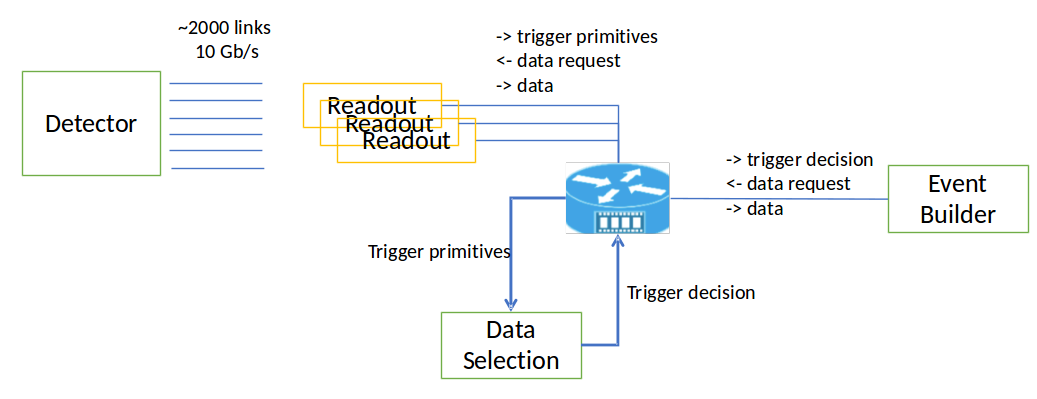
\includegraphics[width=0.8\textwidth]{daq-readout.png}
\end{dunefigure}

The readout system comprises many similar \dword{daqrou}, each connected to a sub-set of electronics from a detector module and interfacing with the \dword{daq} switched network.  Each unit encompasses four functional blocks:

\begin{enumerate}
\item Data reception
\item Network based I/O
\item Data processing
\item Temporary data storage
\end{enumerate}

Each of these blocks are described below.  In addition, and like all other \dword{daq} sub-systems, the readout participates in the common software framework for control, configuration, and monitoring as described in Section~\ref{sec:fd-daq:design-run-control}.

\subsubsection{Data reception}

The physical interface between the detector electronics and the \dword{daq} to transmit data consists of 10 Gbps point-to-point serial optical links, running a simple (e.g., 8/10 bit encoded) protocol. 
The number of links per \dword{dune} module varies from approximately 1000 to 2000, depending on the detector technologies adopted.

To minimize the space and power consumption footprint of the \dword{daq}, 10-20 links are aggregated into \dword{felix} boards hosted in commercial, off-the-shelf computers.
\dword{felix} is an FPGA-based PCIe board developed initially for ATLAS and now proposed or already used in several experiments, including \dword{protodune}. 
Existing firmware will be adopted and adapted to ensure decoding and format checking of incoming data and then to marshal the data to other blocks of the readout sub-system.

\subsubsection{Network based I/O}

The readout system provides access to the data selection and back-end egress systems through a commercial, off-the-shelf switched network as illustrated in Figure~\ref{fig:daq:readout}).
The network communication protocol is as described in Section~\ref{sec:fd-daq:design-messages}.
The network I/O is handled by the \dwords{daqrou} via software; dedicated hardware or firmware development is not required.

\subsubsection{Data processing}

The data processing functional block identifies active areas in the detector (in the TPC and photon detection systems) as a function of time.

As a preliminary step, data may be pre-processed, i.e., organized however best suits subsequent data analysis. This implies reorganizing data into different streams, applying noise filtering algorithms, and compressing and/or zero-suppressing data.

The readout system summarizes the identified detector activity (``hit finding'') on a per-channel basis into information packets called \dwords{trigprimitive}.  These are forwarded to the data selection system which makes correlations and decides whether and which data is to be saved.

This functional block may be implemented onto FPGAs, GPUs, CPUs or a mixture of these elements.
Deciding on the implementation is premature at this stage; this is one of the main topics to explore and develop in the readout area.

\subsubsection{Temporary storage}

In \dword{dune}, the readout system is in charge of temporarily storing all detector data until the data selection system has formed a decision (Section~\ref{sec:sp-daq:design-selection-algs}) on which data to record and until the egress system (Section~\ref{sec:fd-daq:design-backend}) may have sufficient time to request and receive that selected data.
Several time scales and different data throughput metrics dictate the technology and the scaling required to so that this temporary storage is sufficient.

The first time scale is driven by the predominant category of interactions which produces activity that is compact in space and time in the detector. 
The latency to form a \dword{trigdecision} in this case is dominated by processing speed and pipeline depths and is expected to be approximately one second. 
The amount of data that will be requested as a result of such trigger decisions is approximately one or two TPC drift times (5-10\si{\milli\second}, depending on detector technology).

On the other hand, the very rare but important occurrence of a potential \dword{snb} has substantially different and more stringent requirements. 
Potentially, initial activity from an SNB may occur over a period of some seconds which is both too infrequent and of too low energy to form a trigger decision by itself.
However, a subsequent increase in rate of such activity may form an SNB trigger decision. 
It may then be possible to extract important physics information from this early data by employing offline analysis algorithms.
To make it possible to capture that early information the \dword{daq} will continuously buffer at least the prior ten seconds of data.
Then, when a \dword{snb} trigger decision is formed the contents of that buffer will be extracted and eventually output by the DAQ.

Even more important is the data subsequent to the \dword{snb} trigger decision which will span some duration of the main rise and fall of the expected interaction rate signature. 
Capturing both the pre-- and post--trigger data, the \dword{daq} will record a minimum of 30 seconds of data around a \dword{snb} trigger decision. 
The data rates and volumes involved in satisfying these requirements are such that different technology and scale of element must be  used compared to what is required for temporarily storing the more compact interactions.

The worst-case temporary storage requirement for the readout system (using SP detector technology as a metric) is approximately 100 TB per \dword{dune} detector module with a throughput of approximately 10 Tb/s.
This is challenging but technically achievable with current technologies, given suitable granularity of the \dwords{daqrou}. 

In this area, requirements will still need refinement during the detailed design phase of the \dword{daq} system, taking into account the ability to partly compress data as well as more realistic estimates on trigger decision latency, etc.


% \metainfo{Describe how FELIX hardware defines an interface which common to all modules.  Describe how the hardware may handle UDP or other prototocols including bidirectional communication.  Describe how FELIX can be scaled to accept data across a spectrum in order from large to small data rate: the full SP data from the WIBs, full compressed data from the DP, trigger primitive stream from FPGA based units placed between WIBs and FELIX.}


% \ifdp
% \subsubsection{DP data ingest via UDP}
% \label{sec:dp-daq:design-udp-ingest}
% \fixme{dual-phase module, move to DP \dword{daq} chapter eventually}
% \metainfo{This is a DP section and will be only in the DP volume. 
%   It should describe the ``Bump On Wire'' from the IDR unless we can
%   come up with any new/better ideas.}
% \metainfo{Include full hardware scope starting at fibers from CE and
%   ending at the output of trigger processors and the interface between
%   buffer and the Data Selector.
%   Describe the per-APA multiplicity of computers, CPU cores, host
%   system RAM, host system storage, FELIX boards, DPM components (RAM,
%   SSD). 
%   Include thermal estimates itemized by components.}  
% \fi

% \subsection{Front-end Data Handling and Processing}
% \label{sec:sp-daq:design-fe-processing}

% \metainfo{This section describes four functional blocks: (1) 10s RAM buffer (minimum), (2) non-volatile SNB buffer for 30s of data once per month (minimum), (3) hardware for the production of trigger primitive including any data formatting and DPS filtering and (4) compression of selected data.  Note, actual algorithms for trigger primitives are described in Section~\ref{sec:sp-daq:design-selection-algs}.}

% \metainfo{One or two sentences that positions the two processing
%   patterns (FEDHP either before or after FELIX) in this section as options. 
%   Say that the ``FPGA before FELIX'' option is used for ``baseline costing''.}

% \metainfo{Include a table with one row for each known compression factor: \dword{protodune} RCE and FELIX, MicroBooNE before and after noise filter (see docdb), 35t, \dword{protodune} data after ADC stuck code mitigation or avoidance, simulations.  One column of this table shall give a brief comment of how it applies to \dword{dune} including any caveats or reasons for over/under estimation.}

% % \subsubsection{FELIX+FPGA}
% \subsubsection{Upstream FPGA and Firmware}
% \label{sec:sp-daq:design-felix-fpga}
% \fixme{single-phase module}

% \metainfo{Include full hardware scope starting at fibers from CE and
%   ending at the output of trigger processors and the interface between
%   buffer and the Data Selector.
%   Describe the per-APA multiplicity of computers, CPU cores, host
%   system RAM, host system storage, FELIX boards, DPM components (RAM,
%   SSD). 
%   Include thermal estimates itemized by components.}

% % \subsubsection{FELIX+CPU}
% \subsubsection{Downstream CPU and Software}
% \label{sec:sp-daq:design-felix-cpu}
% \fixme{single-phase module}

% \metainfo{Include full hardware scope starting at fibers from CE and
%   ending at the output of trigger processors and the interface between
%   buffer and the Data Selector. 
%   Describe the per-APA multiplicity of computers, CPU cores, host
%   system RAM, SSD and FELIX boards. 
%   Include thermal estimates itemized by components.}


% \subsubsection{Photon Detection System Interface}

% \metainfo{Some motivations for using light to trigger. 
%   (1) want to understand PDS so want to trigger on just the PDS. 
%   (2) background to SNB for which PDS trigger primitives may eliminate. 
%   (3) possibly must rely on light only for SNB triggering, eg if noise is out of control. 
%   Some to all of these should be included.}

% \metainfo{Possibly want to \SI{1}{\micro\second} packet for every time a 1-PE threshold is crossed. 
%   PDS is still understanding what they may send. 
%   \dword{daq} needs to be in control of the trigger forming.}

% \ifdp
% \subsubsection{DP TPC FE issues}

% \fixme{dual-phase module}

% \metainfo{This is similar to SP except for the need to decompress before any trigger primitive processing.  Decompression can potentially happen on FELIX FPGA or on CPU.  There shall be a table or description of the amount of processing required.}

% \subsubsection{DP SP Issues}
% \fixme{dual-phase module}
% \fi

\subsection{Data Selection}
\label{sec:sp-daq:design-selection-algs}
%\fixme{single-phase module}
\fixme{There are many studies which could go into this section. Some of this may very likely be moved into one or more tech notes and referenced.}

The \dfirst{daqdsn} sub-system is responsible for real-time processing
of data from all TPC and PDS subdetectors; using data processing
outcomes and external inputs, it decides
what data must be transferred to the back-end system and
distributes those decisions to the egress sub-system. Data processing
is executed in various stages of firmware and/or 
software, and the overall sub-system is designed to
provide flexibility on where the core processing payload functionality
resides (hardware, firmware, or software). 

The sub-system must select data associated with beam
interactions, atmospheric neutrinos, rare baryon number violating events,
and cosmic ray events depositing visible energy in excess of 100 MeV
with high (targeted at $>$99\%) efficiency. It also must select data
associated with potential galactic supernova bursts, indicating that
the data selection sub-system must be able to self-trigger on
galactic supernova bursts with galactic coverage\footnote{Galactic
  coverage is defined as efficiency-weighted probability of galactic supernova
burst} of $>$95\% efficiency. Moreover, to meet the
requirement that the \dword{dune} \dword{fd} maintain a $<$30~PB per yr to permanent
tape, the \dword{daqdsn} sub-system must effectively reduce the generated data
volume by four orders of magnitude, \fixme{I strongly suggest saying "reduce the generated data by a quarter..." instead of using "four orders of magnitude" (mostly because of audience).} and maintain a fake supernova
burst trigger rate of less than \num{1} \fixme{I also suggest spelling out the number here--numbers from 1-10 should be spelled out.} per month.

The \dword{daqdsn} sub-system design follows a hierarchical structure, where low-level
decisions are fed forward into higher-level ones until a  module-level trigger is activated. The hierarchy
is illustrated in Figure~\ref{fig:daq:data-selection}. The structure
has four levels of processing: Trigger Primitive Generation;
Trigger Candidate Generation; Module Level Trigger; and High Level
Trigger. Each is described in subsequent sections.

\begin{dunefigure}{fig:daq:data-selection}{Block diagram of \dword{dune} \dword{daq}
    Data Selection sub-system, illustrating hierarchical structure of
    sub-system design.}
  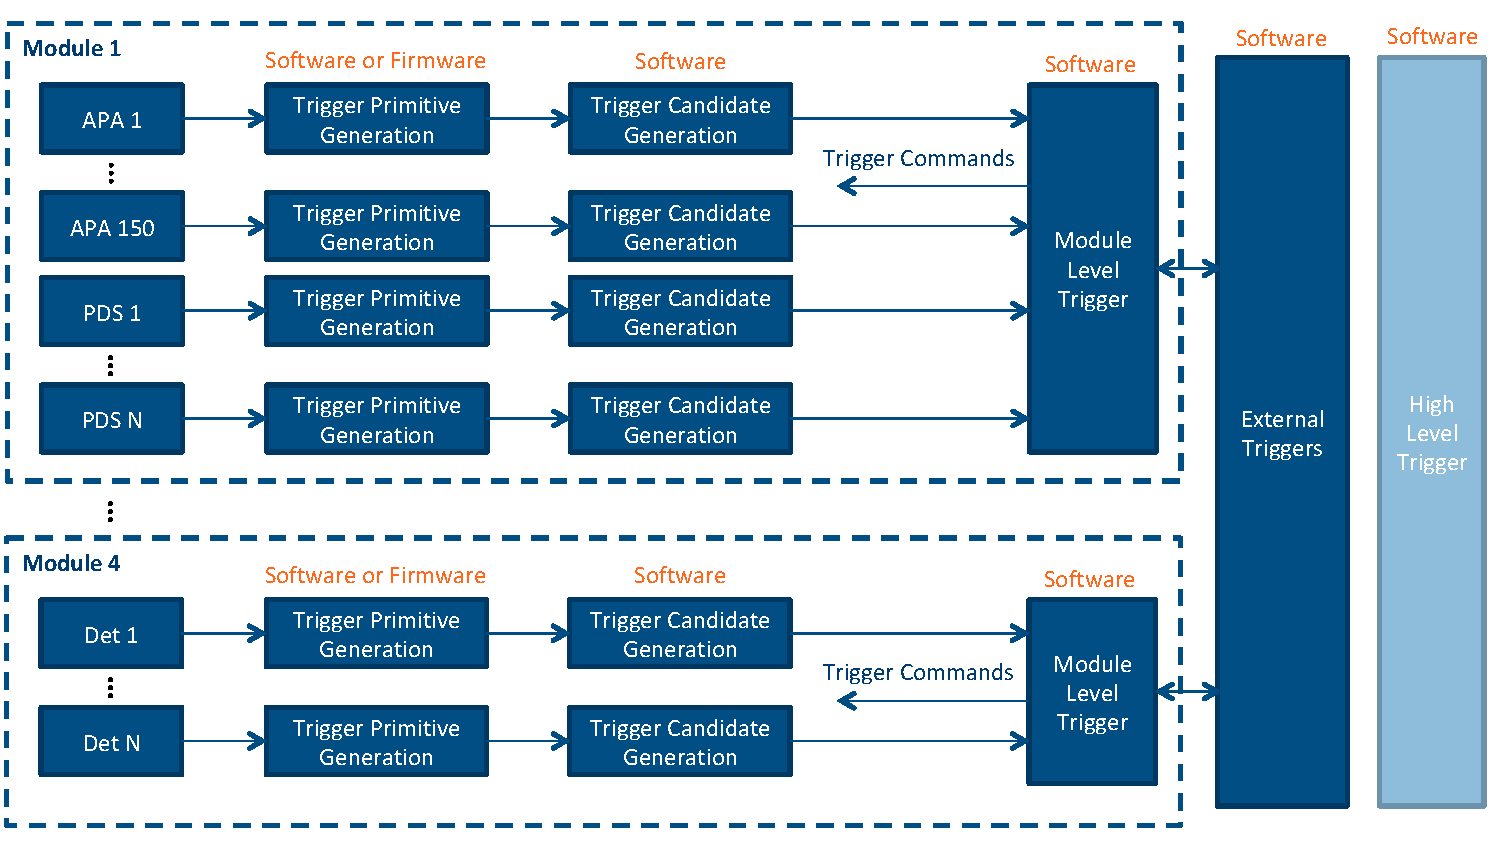
\includegraphics[width=0.8\textwidth]{DUNE_TDR_SP_DAQ_DS_Figure.pdf}
\end{dunefigure}

The first
stage of operations will have two general classes of trigger decisions:
\begin{itemize}
 \item Localized (in time and space) activity triggers: These are
   low-latency triggers intended to prompt readout of
   high-energy events (depositing $>$100~MeV of visible energy) 
   and could also prompt readout of low-energy events
   (e.g., from solar neutrino interactions). In association with a
   localized trigger, a total of minimum two drift windows worth of data is recorded from
   the entire 10-kton module that generated the trigger from
   both TPC and PDS subsystems. \fixme{I read this as "...a minimum total of two drift windows..."}  
\item Extended (in time and space) activity triggers: These are
  high-latency (but no more than 10 seconds) triggers intended to prompt readout of
  activity associated with supernova bursts. This activity spans multiple
  tens of seconds \fixme{How long is multiple tens of seconds?} comprising several supernova neutrino
  interactions as part of an approximately 10-second burst (from a few to
  thousands of interactions for a galactic supernova
  burst). Associated with an extended trigger, a total of \num{100}
  seconds worth of data is recorded from the 10-kton module that
  generated the trigger, including both TPC and PDS subsystems, as
  well as from the other three 10-kton modules, whether
  the latter have generated an extended trigger of their own or not.  
\end{itemize}

To facilitate partitioning, the data selection sub-system must also be
informed and aware of detector configuration and conditions in real
time and apply certain masks on subdetectors or components
in its decision making. It must also provide the Egress sub-system with a list of
subcomponents to read out in association
with any module-level trigger.

\subsubsection{Trigger Primitive Generation}
\label{sec:sp-daq:design-trigger-primitives}
\fixme{single-phase module}

A trigger primitive is defined nominally per-channel and,
in the case of the SP TPC, identified with a per-collection-wire
hit. Trigger primitives provide summary information
like the start time of the pulse on a collection wire, the total
charge or peak of the collection-wire pulse, and the time the pulse
remains above some pre-determined threshold. Trigger primitives for the
TPC are generated in the front-end readout part of the \dword{daq} 
system, either in FPGA firmware or in CPU or GPU software. For the
PDS, TPs are generated in the PDS hardware and streamed to the \dword{daq}
DS sub-system.

Algorithms for generating trigger primitives are still under development
\cite{docid-11275}. An example algorithm is one that a priori \fixme{This is a Latin term and should be in italics.} establishes a
channel baseline, applies baseline subtraction and thresholding, and
identifies a hit over that threshold \cite{docid-11236}. This algorithm has been
validated using both Monte Carlo simulations and real data from \dword{protodune}. Its performance is
summarized in Section~\ref{sec:sp-daq:design-validation}.

Each trigger primitive contains the following information:
\begin{itemize}
\item channel address \[32 bit\]
\item time of hit \[64 bit\]
\item time over threshold \[16 bit\]
\item ADC sum \[32 bit\]
\item error flag \[16 bit\]
\end{itemize}
corresponding to a total of 20 bytes.\fixme{This phrase needs to be attached to an appropriate noun. Is it the trigger primitive that requires 20 bytes? Or is it the information contained in the trigger primitive (that is, the bulleted list) that requires 20 bytes? If the first, this can be phrased "Each trigger primitive, corresponding to a total of 20 bytes, contains the following information:" If the second, this can be rephrased "Each trigger primitive conains the following information, corresponding to a total of 20 bytes:"}

The anticipated trigger primitive rate  will be dominated by
$^{39}$Ar rates (10~MHz per module). Assuming the above \fixme{Where is this? ...the TP format described on page xx...} TP format
prescription, the anticipated trigger primitive rate should \fixme{You may want to do a search for all "is expected to". Most can be replaced with "should" or another auxiliary verb.} be
200~MB/s. The subsequent stage of the DS must absorb and
process this TP rate in real time, providing trigger candidate decisions. 

\metainfo{Include plot and discussion of \dword{dune} trigger primitive rate in \dword{protodune}. 
  The fact that this includes many more cosmics will not matter much as the rate is expected to be dominated by Ar39. 
  Phil has this already but the LAr purity is not yet high enough to see Ar39 across the whole drift distance.}

\subsubsection{Trigger Candidate Generation}

Trigger primitives are streamed from the front-end \dword{daq} readout to a
higher level of data selection that examines those on a per
subdetector (e.g., per APA) basis. This higher level of data selection decides
whether primitives from that subdetector constitute a potential
trigger candidate. Trigger candidates are generated by looking for
clusters of several hits in a narrow time window, the total ADC sum of one or a
cluster of hits, or a large time-over-threshold. Trigger 
candidates will be generated with both a low- and high-energy threshold. The former
will be used for supernova burst triggering, the latter for triggers on beam, atmospheric
neutrinos, cosmics, and other high-energy interactions in the detector. 

A trigger candidate includes not only timing and subdetector
identifier information, but also a rudimentary estimate of the detector
activity that led to the candidate's formation, so that further downstream (at
the module level trigger stage), a decision can be made on 
whether a particular trigger candidate should be counted as part of a possible supernova
burst or a different type of trigger. For example,
a candidate with an estimated energy of 100~MeV would be considered a
localized high energy trigger, while
one with an estimated energy of 5~MeV would only be considered as potentially part of a
supernova burst.\fixme{The second part of this sentence is not entirely clear.}

\subsubsection{Module Level Trigger}
Trigger candidates are passed upstream to a module level trigger that collects candidates
and makes the final decision on what has occurred: a valid localized high-energy
activity (necessitating a module-wide readout trigger for a relatively
short, two-drift duration) or a possible supernova burst (necessitating a module-wide readout
trigger for 100 seconds). The module level trigger passes
trigger Commands, via the Egress sub-system, down to the front-end \dword{daq}
readout, prompting a readout of a pre-determined amount of data depending
on what type of module level trigger has occurred. 

The module level also takes inputs 
from an external trigger, including information from other
modules, SNEWS alerts, and other external signals such as
calibrations. 
It also sends information to the external trigger so that other modules or
detectors can be triggered.

\subsubsection{High Level Trigger}

The last processing stage in the data selection sub-system is the high
level trigger (HLT), \fixme{I believe this needs to be defined in the Dune list of terms? If so, a search and replace can take care of the further use of this abbreviation.} which resides in the
back-end part of the \dword{daq} and is further described in
Section~\ref{sec:fd-daq:design-data-reduction}. The high level trigger
acts on events that have already been triggered, read out, 
and built by the event builder and serves several purposes. It
limits the total triggered data rate that goes to disk by
applying more refined selection criteria to remove events that are clearly uninteresting. For example, instrumentally-generated events
(e.g.~correlated noise) might generate trigger candidates and a module
level trigger, which, upon inspection, can be clearly seen
as non-physics events. Second, it can also reduce the triggered
data set by further identifying and localizing interesting activity.

Beacuse the HLT is in the \dword{daq} back-end and operates on event-built data, for which the rate
should be low, developing more sophisticated
algorithms to eliminate empty APAs from the data 
stream is possible.

\subsection{Back-end System}
\label{sec:fd-daq:design-backend}
\fixme{module-generic}

The \dword{daq} back-end system conceptually encompasses the egress subsystem and interfaces to the buffer and trigger sub-systems shown in Figure~\ref{fig:daq-conceptual-overview}. 
It accepts trigger commands produced by the data selection system as described in Section~\ref{sec:sp-daq:design-selection-algs}. 
It queries the front-end buffer interfaces and accepts returned data as described in Section~\ref{sec:fd-daq:readout}. 
Finally, it records trigger commands and the corresponding data to the output storage buffer, which is then transferred to offline data custody.

\subsubsection{Dataflow Orchestration}

To minimize data extraction latency, the back-end egress sub-system must not serially execute trigger commands to completion. 
This asynchronous execution is termed \dword{daqdfo} and shall operate as illustrated in Figure~\ref{fig:daq:backend} and discussed here:

\begin{dunefigure}{fig:daq:backend}{Illustration of \dword{dune} \dword{daq} back-end operation.}
  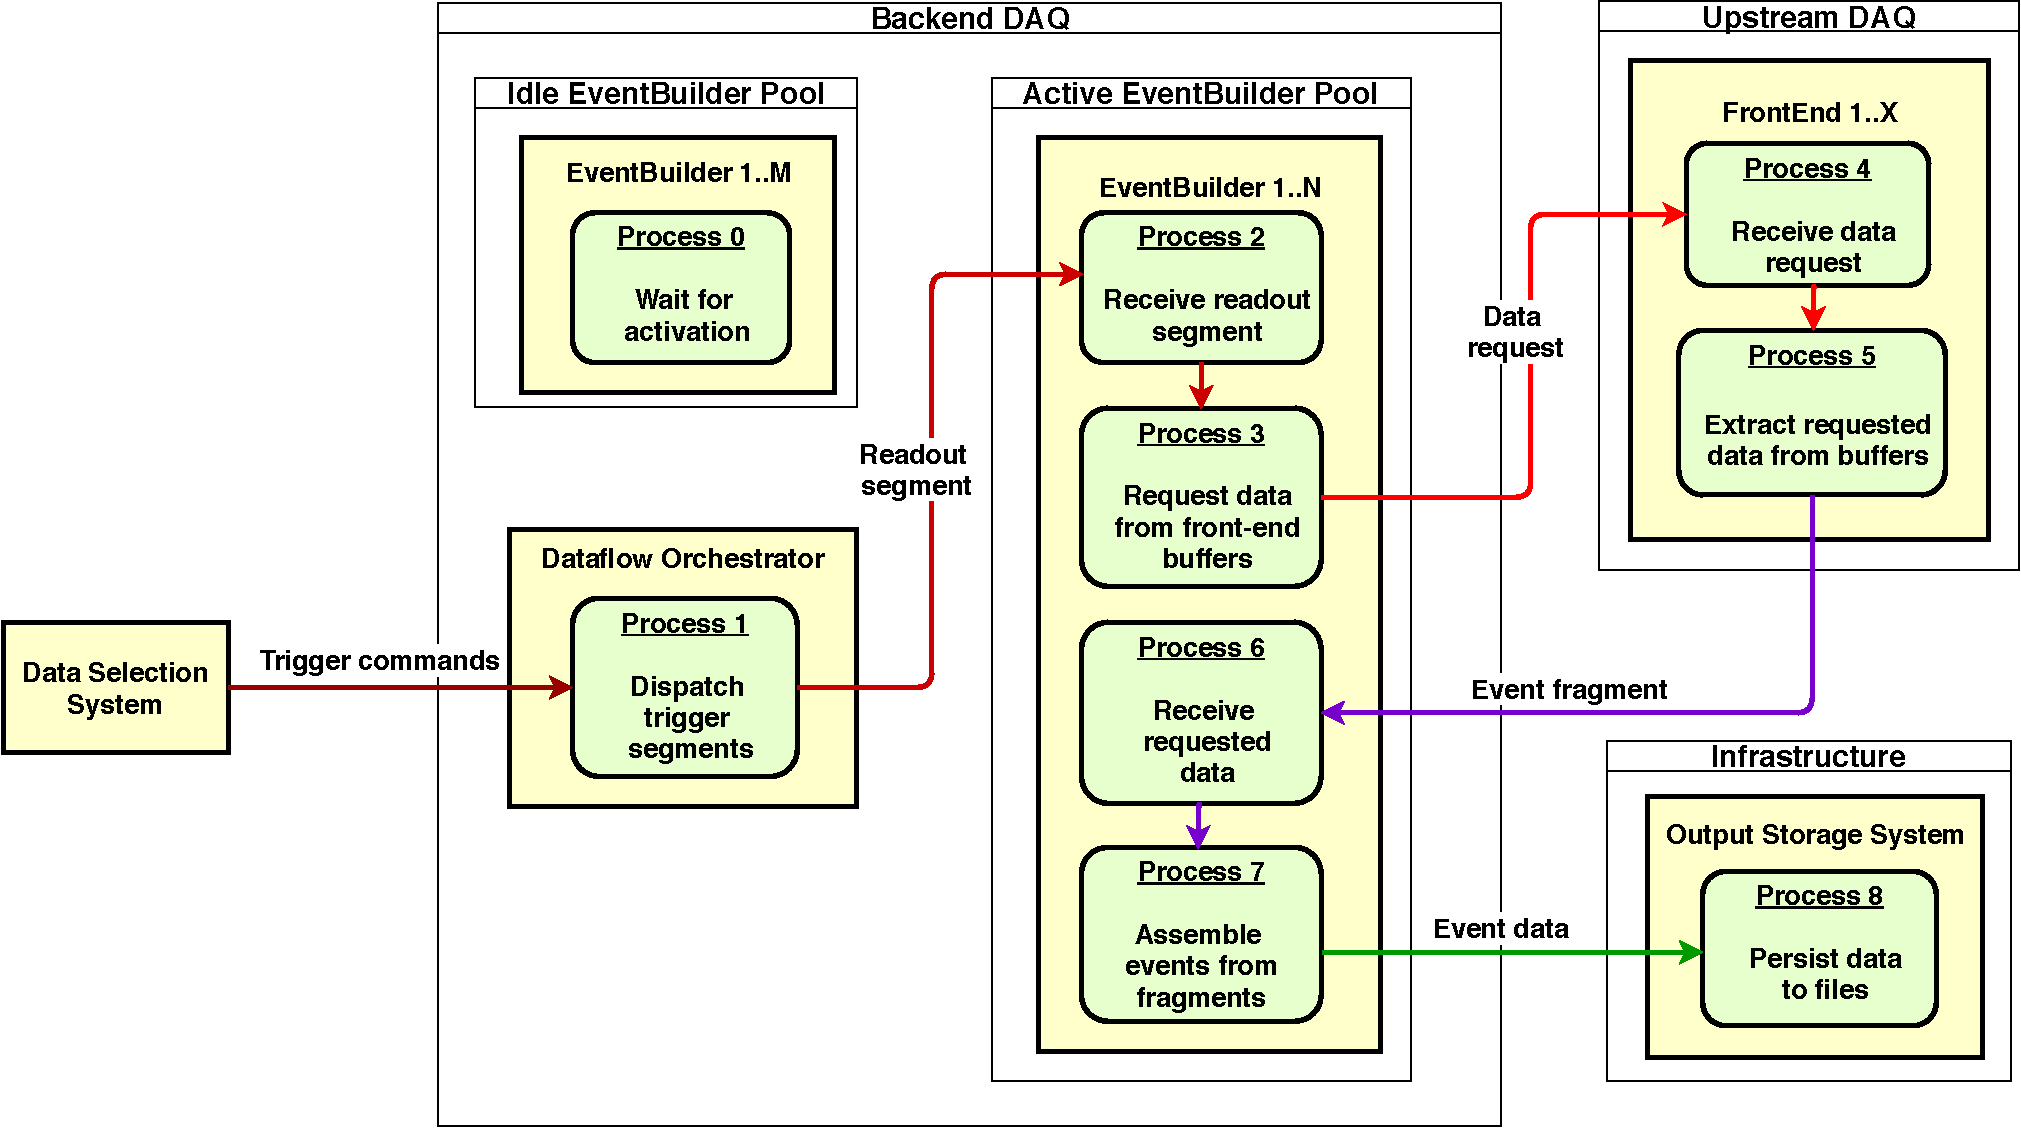
\includegraphics[width=0.8\textwidth]{daq-backend.pdf}
\end{dunefigure}

\begin{itemize}
\item \dword{daqdfo} shall accept a stream of time ordered trigger commands and shall dispatch each for execution.
\item It may evaluate the scope of a trigger command against a configurable set of constraints and segment it into several commands that contiguously and without overlap span the original command.
\item Each trigger command segment shall be dispatched to a process, termed an \dword{eb} as described in Section~\ref{sec:fd-daq:design-event-builder} for execution.
\item \dword{eb} shall execute trigger command segments by requesting data covering the time period and detector span addressed by each trigger command segment.
\item Requests shall be made to the all associated \dwords{daqfbi}, \fixme{I see in the preview that the word interfaces has two S's. This should be fixed.} and the \dword{eb} may expect a response from all even if the buffer has already purged the requested data.
\item The returned data may undergo processing and further aggregation.
\item The returned data shall be saved to one or more files on the output storage system before custody is transferred offline.
\end{itemize}
\fixme{Add time order requirement on DS above}
\fixme{Add return-empty-response requirement to buffer above}



\subsubsection{Event builder}
\label{sec:fd-daq:design-event-builder}
\fixme{module-generic}

\metainfo{Explain art\dword{daq}, handling of trigger commands by asynchronous, parallel queries to front end Data Selector (but take care not to duplicate between here and in the overview).}

The \dword{daq} back-end subsystem shall provide instances of the \dfirst{eb} that requests data from the \dfirst{daqfbi} addressed by a consumed trigger command segment.  An \dword{eb} shall send the returned data to the output storage system.  It may additionally process this data to reduce the amount of data (Section~\ref{sec:fd-daq:design-data-reduction}) and monitor quality (Section~\ref{sec:fd-daq:design-data-quality}) while the data are in flight. 
Resulting output files shall use data schema and file formats as described in Section~\ref{sec:fd-daq:design-data-model}.


\subsubsection{L2 Data Reduction}
\label{sec:fd-daq:design-data-reduction}

To keep efficiency high in collecting information on activities of interest while minimizing selection and content bias and reducing output data rate, we will need high level data reduction processing. 
Called second-level (L2) data reduction, it follows from the first-level provided by the data selection system described in Section~\ref{sec:sp-daq:design-selection-algs}.
To fully understand how much and what type of data reduction may be beneficial, simulation studies performed during preparation for construction and initial data analysis after operation may be necessary. 
The \dword{daq} back-end sub-system thus shall allow for some form of L2 processing although its scale has not been determined. 
The back-end subsystem should help in offline development of processing modules and make porting or directly applying them to the back-end processing system much easier.



\subsubsection{Data Quality Monitoring}
\label{sec:fd-daq:design-data-quality}

Section~\ref{sec:daq:design:ccm:monitoring} described a monitoring system for the \dword{ccm} sub-systems. 
Monitoring the quality of the information held in the detector data itself is critical to promptly responding to unexpected conditions and maximizing the quality of acquired data. 
We must develop a system for continuously processing a subset of the detector data and promptly providing summaries for human consumption; this system is called \dword{daq} \dfirst{dqm}.
The exact suite of products will evolve, and the \dword{dqm} subsystem shall be designed to make this evolution easier. 
Many software modules will be developed offline, so the \dword{dqm} subsystem shall facilitate their reuse when applied to samples of detector data.


\subsubsection{Data Model}
\label{sec:fd-daq:design-data-model}
\fixme{module-generic}

\metainfo{Describe the data model. 
  This isn't a strict schema just things like how various parts of the
  detector readout map to files, etc.}

\subsubsection{Output Buffer}

\metainfo{Describe the output buffer system, how it's shared with offline, data hand-off prototocols.  Responsibility scope (eg, who handles transfer to FNAL).}

The output buffer system is a hardware resource provided by \dword{daq} and used offline by \dword{dune}. 
It has two primary purposes. 
First, it decouples producing content in operating \dword{daq} from transferring that content from the far site to archive storage units and offline processing. 
Second, it provides local storage sufficient for uninterrupted \dword{daq} operation in the unlikely event that the connection between the \dword{fd} and the Internet is lost. 
Based on very unusual losses of connectivity at major laboratories as well as \dword{fd} sites of other long-baseline neutrino experiments, the output buffer shall provide enough storage capacity to retain one week of output given nominal data production. 
The maximum data production rate for the \dword{fd} is set at \SI{30}{\peta\byte/\year}. 
Thus, the output storage buffer must have a capacity of approximately \SI{0.5}{\peta\byte} to service the entire \dword{fd}.
\fixme{How to reference the 30PB/yr requirement?}




\subsection{Timing Distribution and Synchronization System}
\label{sec:sp-daq:design-timing}
%\fixme{single-phase module}
%\fixme{Is it indeed still single-phase specific?}
%\metainfo{Hardware, consumers, links.}

All components of the \dword{fd} use clocks derived
from a single GPS disciplined source, and all module components
are synchronized to a 62.5 MHz clock. To make full use of the
information from the photon detection system (PDS) \fixme{Should this abbreviation go into the set of overall Dune abbreviations?} , the common clock
must be aligned within a single detector unit with an accuracy of
O(1ns) \fixme{I can't tell if this is an O or a zero. I see another few instances of this later.} . For a common trigger for a supernova neutrino burst
(SNB) \fixme{Another abbreviation that may need to be in the overall definitions.} between detector modules, the timing must have
an accuracy of O(1ms). However, a still tighter constraint is
the need to calibrate the common clock to universal time (derived from
GPS) \fixme{Another abbreviation here that is not in LATEX form.} so the data selection algorithm can be adjusted inside an
accelerator spill, which again requires an absolute accuracy of O(1$\mu$s).

The \dword{dune} \dword{fd} uses a version of the \dword{protodune} timing
system, where a design principle is to transmit synchronization messages over
a serial data stream with the clock embedded in the data. The format
is described in \cite{docid-1651}. The timing system design is
described in detail in \cite{docid-11233}.

Central to the timing system are four types of signals:
\begin{itemize}
\item a 10 MHz reference used to discipline a stable master clock,
\item a one-pulse-per-second (1PPS) signal from the GPS,
\item an NTP signal providing an absolute time for each 1PPS signal, and
\item an inter-range instrumentation group (IRIG) time code signal
  used to set the timing system 64-bit time stamp.
\end{itemize}
The timing system relates its time counter onto GPS \fixme{I read this as "The timing system correlates its time counter to GPS time by timestamping..."} time by
timestamping the 1 PPS signal onto its own clock and reading
the corresponding time in software in NTP time.

The timing system synchronization codes are distributed to the \dword{daq}
readout components in the CUC and the readout components on the
cryostat via single mode fibers and passive splitters/combiners. All
custom electronic components of the timing system are contained in two
$\mu$TCA shelves; at any time, one is active while the other serves as
a hot spare. The 10 MHz reference clock and the 1PPS signal
are received through a single-width advanced mezzanine card (AMC) at the
center of the $\mu$TCA shelf. This master timing AMC is a custom board
and produces the timing system signals, encoding them onto
a serial data stream. This serial datastream \fixme{Is data stream one word or two?} is distributed over a backplane to 
a number of fanout AMCs. The fanout AMC is an off-the-self board
with two custom FPGA mezzanine cards (FMCs). Each FMC has four SFP
cages where fibers connect the timing system to each detector
component (e.g., APA) or where direct attach cables connect
to other systems in the CUC.

To provide redundancy, two independent GPS systems are used,
one with an antenna at the surface of the Ross shaft, and the other
with an antenna at the surface of the Yates shaft. Signals from either
GPS are fed through optical single mode fibers to the CUC, where
either GPS signal can act as a hot spare while the other is active. 

\subsection{Design Validation and Development Plan}
\label{sec:sp-daq:design-validation}
\fixme{single-phase module}

The \dword{dune} \dword{fd} \dword{daq} design will be validated and developed using the following strategy:
\begin{itemize}
\item Use \dword{protodune} as a design demonstration platform. 
\item Use Vertical Slice Teststands for further development and testing of
  individual \dword{daq} sub-systems and for key aspects of the
  overall \dword{daq}. 
\item Use \dword{fd} MonteCarlo simulations and studies to augment
  demonstrations using \dword{protodune} and the testing at Vertical Slice Teststands.
\item Cross-check against developments and measurements from other ongoing
  LArTPC experiments.
\end{itemize}

This strategy reflects the current DAQ project schedule, which
comprises several phases, including an intense development phase
running through 2020 that culminates in an engineering design
review (EDR) in Q4 of 2020. At this milestone, the system design will be
finalized and shown to be capable of meeting the requirements of the
final \dword{daq} system. After the development phase, a
pre-production phase begins and will end with a production readiness
review (PRR). By then, final designs of all components
will be complete.

The following subsections summarize past, ongoing, and planned
development and validation studies and identifies how anticipated outcomes
will be used to finalize the \dword{daq} design.
%  Put each validation study (performed or future) in a subsubsection
 % and describe either \textbf{how it justifies a decision} or
 % \textbf{how its outcome will be used to make a decision in the
  %  future}.}

\subsubsection{Ongoing FELIX Throughput Demonstration at \dword{protodune}}
\label{sec:sp-daq:validation-pdune-felix}
%\fixme{single-phase module}

%\metainfo{Describe how the FELIX \dword{daq} at \dword{protodune} demonstrates a
 % FELIX+CPU approach. 
 % Describe the elements that are same or similar (full-rate to host
 % RAM buffer) and different (higher-rate but external trigger).}

The FELIX \dword{daq} at \dword{protodune} partly demonstrates the front-end readout scheme for
the PDS system, as well as the FELIX+CPU readout approach for the
TPC. The elements of the \dword{protodune} FELIX \dword{daq}, which are the
same in \dword{dune}, have already demonstrated the
reception of raw data at full rate from a single APA to a 
FELIX card and FELIX host RAM buffer; upon receiving an external trigger, the
data is propagated to the back-end system. The back-end system
operates similarly to \dword{dune} itself. What differs in the final \dword{dune}
implementation is that in the host CPU or
GPU, nor in the added FPGA functionality, data processing does not trigger primitive generation and subsequent processing
of trigger primitives through the data selection system. Another
significant difference is the much higher rate of data propagation from the
host RAM to the back-end system in \dword{protodune}, which is anticipated to be lower for \dword{dune}. Future development
will concentrate on data processing and data selection.  This is described in more detail in Section~\ref{sec:sp-daq:validation-pd-demonstrator}.

\subsubsection{Ongoing RCE Throughput Demonstration at \dword{protodune}}
\label{sec:sp-daq:validation-pdune-rce}
%\fixme{single-phase module}

The RCE \dword{daq} in \dword{protodune} demonstrates part of the readout scheme for
the FELIX+FPGA readout approach for the TPC. In particular, it
shows that real-time TPC data processing for lossy
and lossless compression can be facilitated in FPGA, achieving
compression factors consistent with those expected based on observed
\dword{protodune} noise levels. In the future, the system will be used
to demonstrate how trigger primitives are generated in FPGA as
described in Section~\ref{sec:sp-daq:validation-pd-demonstrator}.

\subsubsection{Validation of Trigger Primitives in Software}
\label{sec:sp-daq:validation-software-trigger-primitives}
%\fixme{single-phase module}

Generating trigger primitives in CPU or GPU software has not
yet been demonstrated in situ \fixme{This is a Latin term that may need to be in italics.} in \dword{protodune}, but it has been
demonstrated in simulations, using real data from \dword{protodune}, on a
server with specs similar to those 
of the FELIX host server at \dword{protodune}.

The algorithm is described in detail in \cite{docid-11236}; a Monte Carlo test has demonstrated the algorithm can do real-time processing of one APAs worth
of collection wire data. This test was performed on a Xeon Gold 6140
system, where four (4) threads (cores) were sufficient to keep
up with the detector data rate. The algorithm begins with pedestal removal by
finding the mean of any given wire waveform baseline using a frugal
streaming approach. A look-ahead approach was used to stop
updating the pedestal when it became clear that a potential signal
had been found. Noise filtering in the form of a 7-tap low-pass FIR
filter will be applied as an intermediate step
between pedestal subtraction and hit finding. The hit finding
algorithm is a simple threshold-discriminator. Using Monte Carlo, a hit
threshold of 10 ADC counts, corresponding to 1\/4 MIP for deposits originating at the cathode, yields hit primitives dominated by
$^39$Ar and maintains 100\% efficiency to MIP hits. This is robust against noise level 
increases of 50\% above the default \dword{dune} Monte Carlo settings \cite{docid-11275}. 

Tests of trigger primitive generation on very early \dword{protodune} data have also been
performed. Because of its surface
location and the known noisy channels included in this study,
\dword{protodune} trigger primitive generation rates level off to a floor rate higher than a threshold
of approximately 16 ADC counts. Although the total rates are much higher than
anticipated for DUNE, the algorithm performance is promising and should improve as ProtoDUNE \fixme{LATEX form?} continues
to run and improve its noise understanding.

\subsubsection{Validation of Trigger Primitives in Firmware}
\label{sec:sp-daq:validation-firmware-trigger-primitives}
%\fixme{single-phase module}

While trigger primitive generation in firmware has not yet been
demonstrated in the RCE system in \dword{protodune}, candidate
algorithms are being developed and will be deployed in FPGA
for both \dword{protodune} and other demonstrators. 

On the other hand, MicroBooNE has been able to
successfully implement dynamic baseline estimates and subtraction
for region-of-interest (hit) finding in FPGA \cite{NNN18}.
%\metainfo{Succinctly describe algorithm, include physics and computing
%  performance numbers.}

\subsubsection{Validation of Trigger Candidates in Software}


\subsubsection{Validation of High Level Trigger in Software}


\subsubsection{Prototype Message Passing System}
\label{sec:fd-daq:validation-demonstrators}
\fixme{module-generic}

\metainfo{This is actually module-generic. 
  Very briefly describe the prototype message passing. 
  This will mostly refer to a tech note.}


\subsubsection{Planned \dword{protodune} \dword{daq} Demonstrator}
\label{sec:sp-daq:validation-pd-demonstrator}

A demonstration of the DAQ system design based in \dword{protodune} is
planned for 2020. The key components are the front-end readout, timing
system, and data selection systems. A full vertical slice through the
timing and readout system will be constructed, with
TPC and PDS detectors, as well as calibration systems. Although a full-scale
demonstration of the data selection system cannot be achieved with
\dword{protodune}, the basic infrastructure will be demonstrated and
used to self-trigger \dword{protodune}.

The high-level goals will be to demonstrate and validate
\begin{itemize}
\item Integration of Front-End with TPC and PDS electronics;
\item Data throughput for a single front-end instance;
\item Readout data processing for a single front-end instance;
\item Trigger primitive generation for a single front-end instance;
\item Distribution of timing and control signals to detector front-ends;
\item Data selection infrastructure and self-triggering;
\item Integration with calibration systems.
\end{itemize}

The components used in the \dword{protodune}
demonstrator will be assembled in 2019, and their operation will
be verified in standalone tests. For FPGA processing, the
initial version of firmware will be demonstrated in FPGA development
cards, and an integration test will be conducted in 2019 with a
prototype FPGA processing module and the FELIX front-end.


\subsubsection{Planned Vertical Slice Teststands}
\label{sec:sp-daq:validation-demonstrators}
%\fixme{single-phase module}
%\metainfo{Describe VST demonstrators and why we must build them.}

A number of Vertical Slice Teststands will be built to allow
development and testing of individual parts of the \dword{daq} system
as well as testing of key aspects of the design and overall scalability. At minimum, the following teststands
will be constructed:
\begin{itemize}
\item Data Selection: List aims. One option is to construct a
  full-scale data selection system using fake data 
sources, which could be simulated or real (pre-recorded)
\dword{protodune} data,
or both, subject to available resources. Another option is to identify
likely failure points and/or bottlenecks and perform
small-scale tests that stress the critical parts of the corresponding
infrastructrure. The criteria for those tests will be defined a priori /fixme{In this case, I'd suggest not using the Latin term. Use "beforehand" instead.} .
\item Back-end System: List aims.
\end{itemize}

Other than these dedicated Vertical Slice Teststands, a number of
\dword{daq} development kits will be available for other detector and
calibration consortia to support 
their own development, production, and quality assurance programs. The DAQ
kit will also form the basis for testing at the ITF beginning in 2022. This will
also allow validating the detector and \dword{daq} interfaces. %A
%single \dword{daq} kit will be capable of handling data from a single APA. 

\section{Production, Assembly, Installation and Integration}
\label{sec:sp-daq:production}

\metainfo{Describe how hardware, firmware and software will produced. }

\metainfo{Describe how we get stuff in place underground (and in the
  ITF), how we will put it all together and make sure it works. 
  What can we do to minimize the effort needed underground both in
  terms of physical work but also in working out the bugs both in
  individual processes and in emergent behavior of the system as a
  whole?}

\subsection{Computing Hardware}

\subsection{Custom Hardware Fabrication}

\subsection{Software and Firmware Development}
\metainfo{Processes and practices.}

\subsection{ITF}

\section{Cost, Schedule, Safety and Risk Summary}
\label{sec:sp-daq:cost}
\metainfo{
Include cost summary and table here.
Include schedule summary and table here.
Include risk summary and table here.}

\begin{dunetable}
[Data Acquisition System Cost Summary]
{p{0.7\textwidth}p{0.2\textwidth}}
{tab:sp-daq:costsumm}
{Data Acquisition System Cost Summary (made-up numbers)}
 Item & Core Cost (k\$ US) \\ \toprowrule
 (item 1) & \num{67.0} \\ \colhline
 (item 2) & \num{57.8} \\ \colhline
 ... & ... \\ \colhline
 (last item)& \num{47.4} \\
\end{dunetable}

\begin{dunetable}
[Data Acquisition System Schedule]
{p{0.65\textwidth}p{0.25\textwidth}}
{tab:sp-daq:sched}
{Data Acquisition System Schedule (made-up dates)}
Milestone & Date (Month YYYY) \\ \toprowrule
(item 1) & October 2020 \\ \colhline
(item 2) & March 2021 \\ \colhline
... & ... \\ \colhline
(last item)& June 2023 \\
\end{dunetable}


\begin{dunetable}
[Data Acquisition System Risk Summary]
{p{0.15\textwidth}p{0.75\textwidth}}
{tab:sp-daq:risks}
{Data Acquisition System Risk Summary}
ID & Risk \\ \toprowrule
(id 1) & risk text \\ \colhline
(id 2) & risk text \\ \colhline
... & ... \\ \colhline
(last id)& risk text \\
\end{dunetable}